\chapter{Scheme Environment}

Scheme development environment is foundation for number of fascinating applications in education and research. But, executing scheme programs directly into browser is not possible yet, scheme environment is not readily available in browser. In such cases, Java Script being de-facto of browser based applications, a Java Script based, and browser native implementation Scheme environment is desirable.

For this project, we created scheme environment in browser using Java Script. Our scheme interpreter follows R5RS Scheme standards. It provides supports for some of the core language features with additional feature of interacting with DOM to enable scheme to interact with browser.  The core of our environment is inspired by Nashorn \cite{javascripting}. 

\begin{figure}[ht]
	\begin{center}
		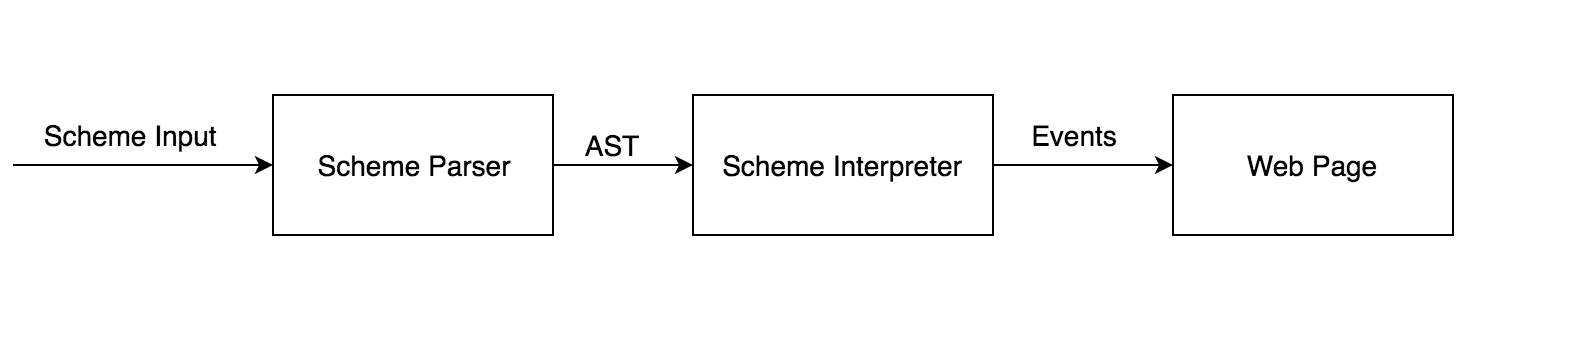
\includegraphics[width=\linewidth]{./images/SchemeEnvironmentusingJavaScript.png}
	\end{center}
	\caption{Scheme Environment using Java Script : Architecture}
	\label{fig:SchemeEnvironmentusingJavaScript}
\end{figure}


As shown in figure \ref{fig:SchemeEnvironmentusingJavaScript}. Our enviroment takes web page embedded scheme script as input, and then depending on approach, it will be parse, and then interpret the input using Java Script. This interpreted  scheme code then interacts with browser, to help render web pages with more dynamic behaviour. 

\section{Interpreter} 
As we discussed in previous chapters, browsers does not have readily available support for scheme. To help enable browser to understand code written in scheme, we built scheme interpreter written in Java Script. Using our scheme interpreter, browser will understand program written in Scheme.

Scheme code will be embedded into web page using script tag as shown in the example below, 

\begin{lstlisting}[frame=single]  
<!DOCTYPE html>
<html>
<head>
<meta charset="utf-8" />
<title>Scheme example</title>
</head>
<body>
</body>
<script type="text/scheme">
	(
		(define square
			(lambda (n) 
				(console-log (* n n)) 
			)
		)
		
		(square 6)
	)

</script>

</script>

</html>
\end{lstlisting}

As shown in the code snippet above, scheme code can be added inside webpage, by writing it between "$<$script type="text/scheme" $>$ $<$/script$>$" tags. Our interpreter supports multiple number of scheme script tags.

In order for browser to understand Scheme, Code snippet written inside this scheme script tags, is parsed and interpreted by our library. For JS library approach, we need to include library reference of interpreter on the page, as shown in example below, 

\begin{lstlisting}[frame=single]  
	<script src="simple-scheme-interpreter.js">
\end{lstlisting}

For browser plugin approach this script file is added by browser plugin, so we don't have to worry about adding it in the web page.

Interpreter consists of two parts discussed in next sections.

\subsection{Parser}

After, code snippets from script tags is read, first thing our library do is to parse the input code and get the Abstract Syntax Tree (AST), which we can then use for interpretation. 

\subsubsection{PEG.js}

To create, parser for scheme, we used PEG.js library. PEG.js is simple parser written in Java Script, We can use to create parsers for complex data, and computer languages. PEG.js grammar used to parse scheme code is shown in code snippet below,

\begin{lstlisting}[frame=single]  
var parser = PEG.buildParser(
' start = multiexpression;\
validchar = [a-zA-Z_?!+\\-=@#$%^&*/.];\
spaces = \" \"*;\
newline = [\\n]*;\
digit = [0-9];\
atom =    spaces newline chars:validchar+ spaces newline   { return chars.join(\"\"); }\
/ spaces newline numbers:digit+ spaces newline     { return parseInt(numbers.join(\"\")); };\
list =    spaces newline \"(\" spaces newline expressionss:multiexpression+ newline spaces\")\"  spaces newline { return expressionss; };\
expressions = spaces newline  lists:list+ newline spaces { return lists };\
multiexpression = atom / expressions ;');
\end{lstlisting}

Using above grammar, scheme code is parsed into AST using following statement,

\begin{lstlisting}[frame=single]  
 var PegAST= parser.parse(s);
\end{lstlisting}


\subsection{Interpreter}

AST generated by the browser is then interpreted by our interpreter written in Java Script as shown in code snippet below.

\begin{lstlisting}[frame=single]  
var pegRet = schemeInterpreter.interpret(PegAST);
\end{lstlisting}

Interpreted output is Java Script code which browser understands.

\section{Scheme for Browser} 

Our implementation scheme used R5RS standard, variable are  blocked scoped in the program. 

Blocks can be created with let, or define expressions, like so:


\begin{lstlisting}[frame=single]  
	(let ((x 10)
		(y 20))
	
	(foo x y))
\end{lstlisting}


In the example, shown above, variable x, and y are blocked scoped, both x and y are available to function foo.

Like universal scheme, our implementation of scheme supports following features- 



\begin{itemize}
	\item {\textbf{Basic Types}}
	\begin{itemize}
		\item Integer
		\item Real
		\item Number
		\item String
		\item List
		\item Char
	\end{itemize}
\end{itemize}

\begin{itemize}
	\item{\textbf{Control structure}}
	\begin{itemize}
		\item Conditional
		\begin{itemize}
			\item if then else cond case
		\end{itemize}
		\item Loop
		\begin{itemize}
			\item do let(named let) dotimes
		\end{itemize}
		\item Assignment
		\item eval
	\end{itemize}
\end{itemize}

It also, provides special language syntax to interact with Browser's DOM. 
This is only available for browser.

\begin{itemize}
	\item {\textbf{Browser  Functions}}
	\begin{itemize}
		\item {Dialog}
			\begin{itemize}
				\item {(alert msg)}
					\begin{itemize}
						\item {$=$ window.alert}
					\end{itemize}
			\end{itemize}
		
			\begin{itemize}
				\item {(confirm msg) =$>$ boolean}
				\begin{itemize}
					\item {$=$ window.confirmt}
				\end{itemize}
			\end{itemize}
	\end{itemize}

	\begin{itemize}
		\item {Event}
		\begin{itemize}
			\item {(add-handler! selector event proc) =$>$ js-handler}
		\end{itemize}
		
		\begin{itemize}
			\item {(remove-handler! selector event js-handler)}
			\begin{itemize}
				\item {eg. (define h (add-handler! "$#$button1" "click" (lambda (ev) ...)))}
				\item {eg. (remove-handler! "$#$button1" "click" h)}
			\end{itemize}
		\end{itemize}
	\end{itemize}

	\begin{itemize}
		\item {Element}
		\begin{itemize}
			\item {(element-visible? elem)}
			\item {(element-toggle! elem)}
			\item {(element-hide! elem)}
			\item {(element-show! elem)}
			\item {(element-remove! elem)}
			\item {(element-update! elem html)}
			\item {(element-replace! elem x)}
			\item {(element-insert! elem x)}
			\item {(element-select elem)}
		\end{itemize}
	\end{itemize}
\end{itemize}

Apart, from providing DOM APIs for browser, our scheme interpreter also, provides, interface to some of the basic Java Script functions as shown below, 


\begin{itemize}
	\item{\textbf{JavaScript language interface}}
	\begin{itemize}
		\item {(js-eval str) evaluate str as JavaScript code}
	\end{itemize}

	\begin{itemize}
		\item Console
		\begin{itemize}
			\item {(console-debug obj1 ...) = console.debug}
			\item {(console-log obj1 ...)}
			\item {(console-info obj1 ...)}
			\item {(console-error obj1 ...)}
		\end{itemize}
\end{itemize}
\end{itemize}


\section{Approches}

Our project implements two approches to help browser able to understand scheme code written in web page.

\subsection{Browser Plugin } 
For this approach, browser plugin (supported by firefox, and chrome) will push the instance of PEG.js parser and our scheme interpreter into every newly opened browser tab. In this way, user don't have to worry about adding the library script on the page. Our library will then parse and interpret all the code enclosed within scheme script.

\begin{lstlisting}[frame=single]  
<!DOCTYPE html>
<html>
<head>
<meta charset="utf-8" />
<title>Scheme Alert example</title>
</head>
<body>
</body>
<script type="text/scheme">
(alert "Hello World")
</script>
</script>
</html>
\end{lstlisting}

As shown in the code snippet above, we don't need to add any external libraries into our webpage, to interpret scheme script. Browser plugin will take care of that.
Executing above code in browser with our plugin installed, will alert user with "Hello World" as text.


\subsection{JS Library}


In this approach, scheme support is achieved in web pages by including scheme interpreter and parser libraries in web page itself. When web page will loaded into browser,  library will read code snippet inside scheme script and will interpret it, as shown in the example below, 


\begin{lstlisting}[frame=single]  
<!DOCTYPE html>
<html>
<head>
<meta charset="utf-8" />
<title>Scheme Alert example</title>
</head>
<body>
</body>

<script src="https://cdnjs.cloudflare.com/ajax/libs/pegjs/0.9.0/peg.js">
</script>
<script type="text/scheme">
	(alert "Hello World")
</script>
<script src="./simple-scheme-interpreter.js">
</script>
</html>
\end{lstlisting}

As shown in code snippet above,  instance of PEG.js and scheme-interpreter is embedded directly into the web page. Interpreter will then interpret "(alert "Hello World") and it will show an alert on the screen with "Hello World" as text.


\section{JS to Scheme Interaction}

